% Preámbulo

% Tipo de documento
\documentclass[a4paper, 12pt]{article}
% Codificación
\usepackage[utf8]{inputenc} 
\usepackage{fancyhdr}
\usepackage{graphicx}
% Idioma
\usepackage[spanish]{babel}
%Tipografía
\usepackage{gfsartemisia}
\usepackage[T1]{fontenc}
\usepackage[usenames]{color}
\definecolor{Lila}{rgb}{0.39,0.17,0.63}
\definecolor{Azul}{rgb}{0.17,0.39,0.63}
%%% Matemáticas Paquetes AMS
\usepackage{amsfonts}
\usepackage{amsmath} % Matemáticas
\usepackage{amssymb,amsthm} % Símbolos y teoremas
\usepackage{mathtools} % % Algunos añadidos y correcciones a amsmath
\usepackage{esvect}
%referencia
\usepackage{hyperref}
% Título y autor de un documento. Fecha. Tabla de contenido
\pagestyle{fancy}
\fancyhf{}
\rhead{Ejercicio de Entrega}
\lhead{Daniel Alconchel Vázquez}
\rfoot{Page \thepage}

%Maths
\theoremstyle{plain}
\newtheorem{teorema}{Teorema}[section]
\newtheorem{coro}[teorema]{Corolario}
\newtheorem{proposicion}[teorema]{Proposición}
\newtheorem{lema}[teorema]{Lema}
\theoremstyle{definition}
\newtheorem{definicion}[teorema]{Definición}
\theoremstyle{remark}
\newtheorem*{observacion}{Observación}

\begin{document}
	\begin{flushleft}
	\textbf{1.} Dado $\alpha > 0$, se considera la ecuación en diferencias
	\[x_{n+1}=1-\alpha\mid x_n\mid\]
	
	a) Para $\alpha=0.7$, estudia gráficamente el comportamientos de las soluciones en función de su dato inicial $x_0 \in \Re$.
	
	b) Para $\alpha> 0$ determina el número de puntos de equilibrio de la ecuación.
	
	c) Estudia la estabilidad de los puntos para $\alpha= 1.8$.
	
	d) Si $\alpha=2$, comprueba que \{-0.2,0.6\} es un 2-ciclo y estudia su estabilidad.
	
	\end{flushleft}

	\bigskip
	Comenzamos considerando la función $f:\Re \rightarrow \Re$ como \\$f(x):=1-\alpha\mid x\mid$, la cual, podemos reescribir como una función a trozos, de la siguiente manera:
	\[f(x)= \left\{ \begin{array}{lcc}
	1-\alpha x &   si  & x \geq 0 \\
	\\ 1+\alpha x &  si & x < 0 \\
	\end{array}
	\right.\]
	Esta función es la que define la recurrencia dada en el enunciado.
	
	Procedemos a calcular su derivada:
	\[f'(x)= \left\{ \begin{array}{lcc}
	-\alpha &   si  & x \geq 0 \\
	\\\alpha &  si & x < 0 \\
	\end{array}
	\right.\]
	
	\textbf{Apartado 1}
	
	Sea $\alpha=0.7$, entonces la función f queda determinada de la siguiente manera:
	\[f(x)= \left\{ \begin{array}{lcc}
	1-0.7 x &   si  & x \geq 0 \\
	\\ 1+0.7 x &  si & x < 0 \\
	\end{array}
	\right.\]
	
	Procedemos a calcular los puntos de equilibrio de la función, para lo que resolvemos la ecuación $f(x) = x$. Como tenemos una función a trozos, tenemos que distinguir dos casos:
	
	\begin{enumerate}
		\item Si $x\geq 0$ tenemos que resolver la ecuación $x=1-0.7x$. Luego, tenemos:
		\[x=1-0.7x \implies 1.7x=1 \implies x=\frac{10}{17}\]
		Como estamos en la región $x\geq 0$, el resultado es válido
		\item Si $x<0$ tenemos que resolver la ecuación $x=1+0.0.7x$. Luego, tenemos:
		\[x=1+0.7x \implies 0.3x=1 \implies x=\frac{10}{3}\]
		Como estamos en la región $x<0$, la solución no es válida.
	\end{enumerate}

	Como el punto $x=\frac{10}{17}$ es un punto de equilibrio de la función f y como $\mid f'(\frac{10}{17}) \mid = \mid -0.7 \mid < 1$, el punto es asintóticamente estable, y, por tanto, si escogemos un valor inicial de $x_0$ que se encuentre dentro de un entorno de $p=\frac{10}{17}$, el sistema convergerá a dicho punto de equilibrio.
	
	La representación gráfica sería la siguiente:
	
	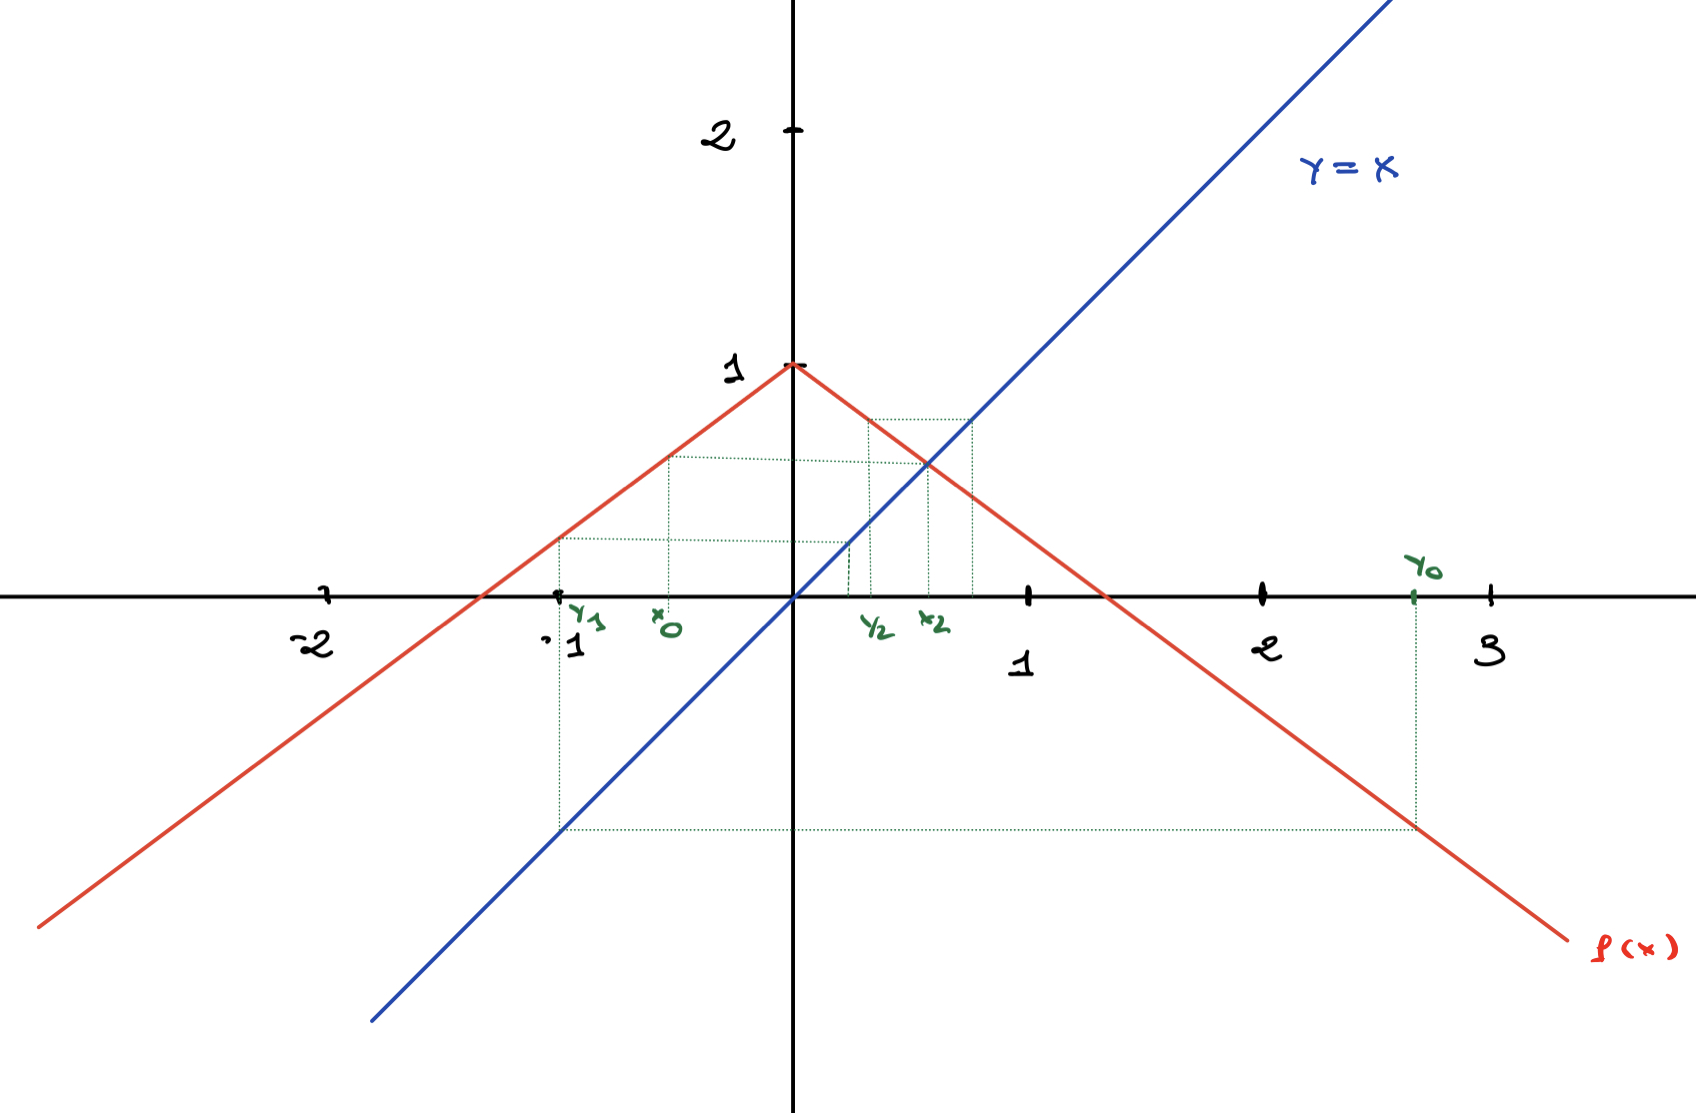
\includegraphics[scale=0.25]{graf}
	
	\textbf{Apartado 2}
	
	Tenemos $\alpha >0$. Recordemos que los puntos de equilibrio se obtienen resolviendo la ecuación $f(x)=x$. Luego, nuevamente, tenemos que distinguir dos casos:
	
	\begin{enumerate}
		\item Si $x\geq 0$ tenemos que resolver la ecuación $x=1-0.7x$. Luego, tenemos:
		\[x=1-\alpha x \implies (1+\alpha)x=1 \implies x=\frac{1}{1+\alpha}\]
		Como estamos en la región $x\geq 0$, el resultado es válido, ya que $\alpha >0$.
		\item Si $x<0$ tenemos que resolver la ecuación $x=1+\alpha x$. Luego, tenemos:
		\[x=1+\alpha x \implies (1-\alpha)x=1 \implies x=\frac{1}{1-\alpha}\]
		Como estamos en la región $x<0$, la solución solo será valida si $x=\frac{1}{1-\alpha}<0 \implies 1-\alpha <0 \implies \alpha > 1$.
	\end{enumerate}

	Luego, tenemos que $\forall \alpha>0$ el punto $x=\frac{1}{1+\alpha}$ es un punto de equilibrio, y que si $\alpha > 1$, también tendríamos el punto $x=\frac{1}{1-\alpha}$.
	
	\bigskip
	\textbf{Apartado 3}
	
	Tenemos $\alpha=1.8$, luego, estamos en el caso $\alpha > 1$, por lo que ,usando el apartado anterior, tenemos que existen dos puntos de equilibrio, que son $x=\frac{1}{1+1.8}=\frac{5}{14}$ y $x=\frac{1}{1-1.8}=\frac{-5}{4}$.
	
	\medskip
	Recordemos que tenemos: 
	\[f'(x)= \left\{ \begin{array}{lcc}
	-\alpha &   si  & x \geq 0 \\
	\\\alpha &  si & x < 0 \\
	\end{array}
	\right.\]
	
	Luego:
	\[f'(x)= \left\{ \begin{array}{lcc}
	-1.8 &   si  & x \geq 0 \\
	\\1.8 &  si & x < 0 \\
	\end{array}
	\right.\]
	
	\medskip
	Por lo que tenemos que $\mid f'(\frac{5}{14}) \mid = \mid f'(\frac{-5}{4}) \mid = \mid 1.8 \mid > 1$. Luego, ambos puntos de equilibrio son inestables.
	
	\bigskip
	\textbf{Apartado 4}
	
	Para $\alpha= 2$ tenemos que:
	\[f(x)= \left\{ \begin{array}{lcc}
	1-2 x &   si  & x \geq 0 \\
	\\ 1+2 x &  si & x < 0 \\
	\end{array}
	\right.\]
	
	\medskip
	Luego, observamos que $f(-0.2) = 0.6$ y $f(0.6) = -0.2$, luego, efectivamente existe el 2-ciclo.
	
	Ahora, para calcular su estabilidad observemos que:
	\[f'(x)= \left\{ \begin{array}{lcc}
	-2 &   si  & x \geq 0 \\
	\\2 &  si & x < 0 \\
	\end{array}
	\right.\]
	
	\medskip
	Luego, tenemos que $\mid f'(0.2)\cdot f'(0.6) \mid= \mid -2\cdot 2\mid = \mid -4 \mid = 4 > 1 $. Luego, concluimos con que el 2-ciclo no es estable.
	
\end{document}